% PAKETE UND DOKUMENTKONFIGURATION
\documentclass[11pt, a4paper]{scrbook}

% Encoding für Umlaute
\usepackage[utf8]{inputenc}
\usepackage[T1]{fontenc}

% Silbentrennung
\usepackage[ngerman]{babel}

% erweiterte Matheumgebungen und Formelnummer mit Sectionnummer
\usepackage{amsmath}

% zusätzliche mathematische Schriftarten
\usepackage{amsfonts}

% verschiedene mathematische Symbole
\usepackage{amssymb}

%
\usepackage{textcomp}
\usepackage{mathtools}

% Einheiten setzen z.B. \SI{10}{\kilo\gram\meter\per\second\squared}
% Fehler: \SI{10 +- 0,2e-4}{\metre}
\usepackage{siunitx}
\sisetup{
  output-decimal-marker={,},
  separate-uncertainty
}

% Bilder einfügen
\usepackage{graphicx}

% Textfarbe
\usepackage[dvipsnames]{xcolor}

% Verweise innerhalb des Dokuments
\usepackage{hyperref}
\hypersetup{
	colorlinks = true,
	allcolors = {black}
}

\newcommand{\vnabla}{\vec{\nabla}}
\newcommand{\ve}{\vec{E}}
\newcommand{\vb}{\vec{B}}
\newcommand{\vh}{\vec{H}}
\newcommand{\vd}{\vec{D}}

\newcommand{\todo}[1]{{\textcolor{Green}{(#1)}}}

\title{Störkörpermessung an Beschleunigungsresonatoren}
\author{Christopher Deutsch}

\begin{document}
	\frontmatter
	\maketitle
	\tableofcontents
	
	\mainmatter
	
	\chapter{Einleitung}
	
	
	\chapter{Theorie}	
	\section{Hohlraumresonatoren}
	Ein Hohlraumresonator besteht aus einem evakuierten Hohlraum, welcher durch ein leitendes Material begrenzt wird.
	Die im Hohlraum propagierenden elektromagnetischen Wellen werden an den leitenden Wänden reflektiert und führen zur Ausbildung von stehenden elektromagnetischen Wellen im Resonatorinnenraum, welche unter anderem zur Beschleunigung von elektrisch geladenen Teilchen genutzt werden können.
	Aufgrund der Randbedingungen an der näherungsweise ideal leitenden Grenzfläche müssen die folgenden Anforderungen an das elektromagnetische Feld gestellt werden:
	\begin{align}
		E_\parallel = 0 \qquad \text{und} \qquad B_\perp = 0\text{,}
		\label{eq:randbedingung_leiter}
	\end{align}
	wobei $E_\parallel$ die Tangentialkomponente und $B_\perp$ die Normalkomponente des elektrischen bzw.\ magnetischen Feldes auf der Grenzfläche kennzeichnet.
	Die Lösung der \textsc{Maxwell}-Gleichungen unter Beachtung dieser Grenzbedingungen zeigt, dass in Abhängigkeit der Geometrie des Hohlraums, eine unbegrenzte Anzahl von Moden mit bestimmten Frequenzen im Resonator auftreten können.
	Die Klassifizierung der einzelnen Moden erfolgt dabei anhand ihrer Feldkonfiguration relativ zur Propagationsrichtung der hin- und rücklaufenden Wellen im Resonator.
	Dabei unterscheidet man zwischen transversal elektrischen (TE)-Moden, welche lediglich transversale elektrische und longitudinal magnetische Felder aufweisen und transversal magnetischen (TM)-Moden, bei denen der umgekehrte Fall eintritt.
	
	Viele der in Beschleunigern verwendeten Kavitäten\footnote{von lat.\ \emph{cavum} "Höhle": Hohlraumresonator oftmals engl. \emph{Cavity}} basieren auf kreiszylindrischen Resonatoren\footnote{engl. \emph{Pillbox-Cavities}, für deren Ähnlichkeit mit einer Tablettenschachtel}, welche eine analytische Lösung der \textsc{Maxwell}-Gleichungen erlauben.
	Daher soll im Folgenden die Feldkonfiguration der verschiedenen Moden am Beispiel der \emph{Pillbox-Cavity} (Abb. ???) dargestellt und die in dieser Arbeit verwendete Notation eingeführt werden.
	Dabei genügt die Betrachtung der longitudinalen Felder eines zylindrischen Hohlraums mit Radius~$R$ und Länge~$L$ in Zylinderkoordinaten $(r, \theta, z)$, da durch diese die transversalen Feldkomponenten eindeutig festgelegt sind \cite{hillert}.
	Man findet für die Moden in dem kreiszylindrischen Resonator \cite{wangler}:
	\begin{subequations}
		\begin{align}
		\mathrm{TM}_{mnp}\text{-Mode:} \quad E_z = E_0 J_m(k_{mn} r) \cos(m \theta) \cos\left(\frac{p \pi z}{L}\right) \exp(i \omega_{mnp} t) \qquad B_z = 0\\
		\mathrm{TE}_{mnp}\text{-Mode:} \quad B_z = B_0 J_m(k_{mn}^\prime r) \cos(m \theta) \sin\left(\frac{p \pi z}{L}\right) \exp(i \omega_{mnp}^\prime t) \qquad  E_z = 0
		\end{align}
		\label{eqs:felder_pillbox}
	\end{subequations}
	wobei die Konstante $k_{mn}^{(\prime)}$ definiert ist als:
	\begin{align}
	k_{mn}^{(\prime)} := \frac{x_{mn}^{(\prime)}}{R}
	\end{align}
	mit der $n$-ten positiven Nullstelle $x_{mn}$ Besselfunktion $m$-ter Ordnung $J_m(x)$ respektive ihrer Ableitung $J_m^\prime(x)$.
	Aus Gleichungen \eqref{eqs:felder_pillbox} folgt dann die Bedeutung der Indizes $m, n$ und $p$:
	Der Index $m$ ($m=0, 1, \dots$) beschreibt die Periodenzahl der Feldkomponente in azimutaler Richtung.
	Weiterhin wird durch $n$ ($n=1, 2, \dots$) die Anzahl der Knoten der longitudinalen Feldkomponente in radialer Richtung (ausgenommen Knoten im Ursprung mit $r=0$) gegeben.
	Schließlich gibt der Index $p$ (TM-Mode: $p= 0, 1, \dots$; TE-Mode: $p = 1, 2, \dots$) die Anzahl der halben Perioden in longitudinaler Richtung an.
	
	Die Kreisfrequenz~$\omega_{mnp}$ der einzelnen Moden ist dabei gegeben durch \cite{wangler}:
	\begin{align}
	\omega_{mnp}^{(\prime)} = c \cdot \sqrt{\left( k_{mn}^{(\prime)}\right)^2 + \left( \frac{p \pi}{L} \right)^2}
	\end{align}
	\todo{Bilder Pillbox, Felder und TM010 im Beschleuniger / Lichtgeschwindigkeit im Medium ?}
	
	Eine analytische Berechnung der Moden von komplexeren Resonatorgeometrien ist nicht mehr möglich und es muss auf numerische Methoden zurückgegriffen werden.
	Dazu wird in dieser Arbeit \emph{CST Microwave Studio\textsuperscript{\textregistered}} verwendet, welches die Lösung der Maxwell-Gleichungen diskretisiert und auf ein Eigenwertproblem zurückführt.
	
	\section{Hohlraumresonatoren2}
	\begin{figure}[h]
		\centering
		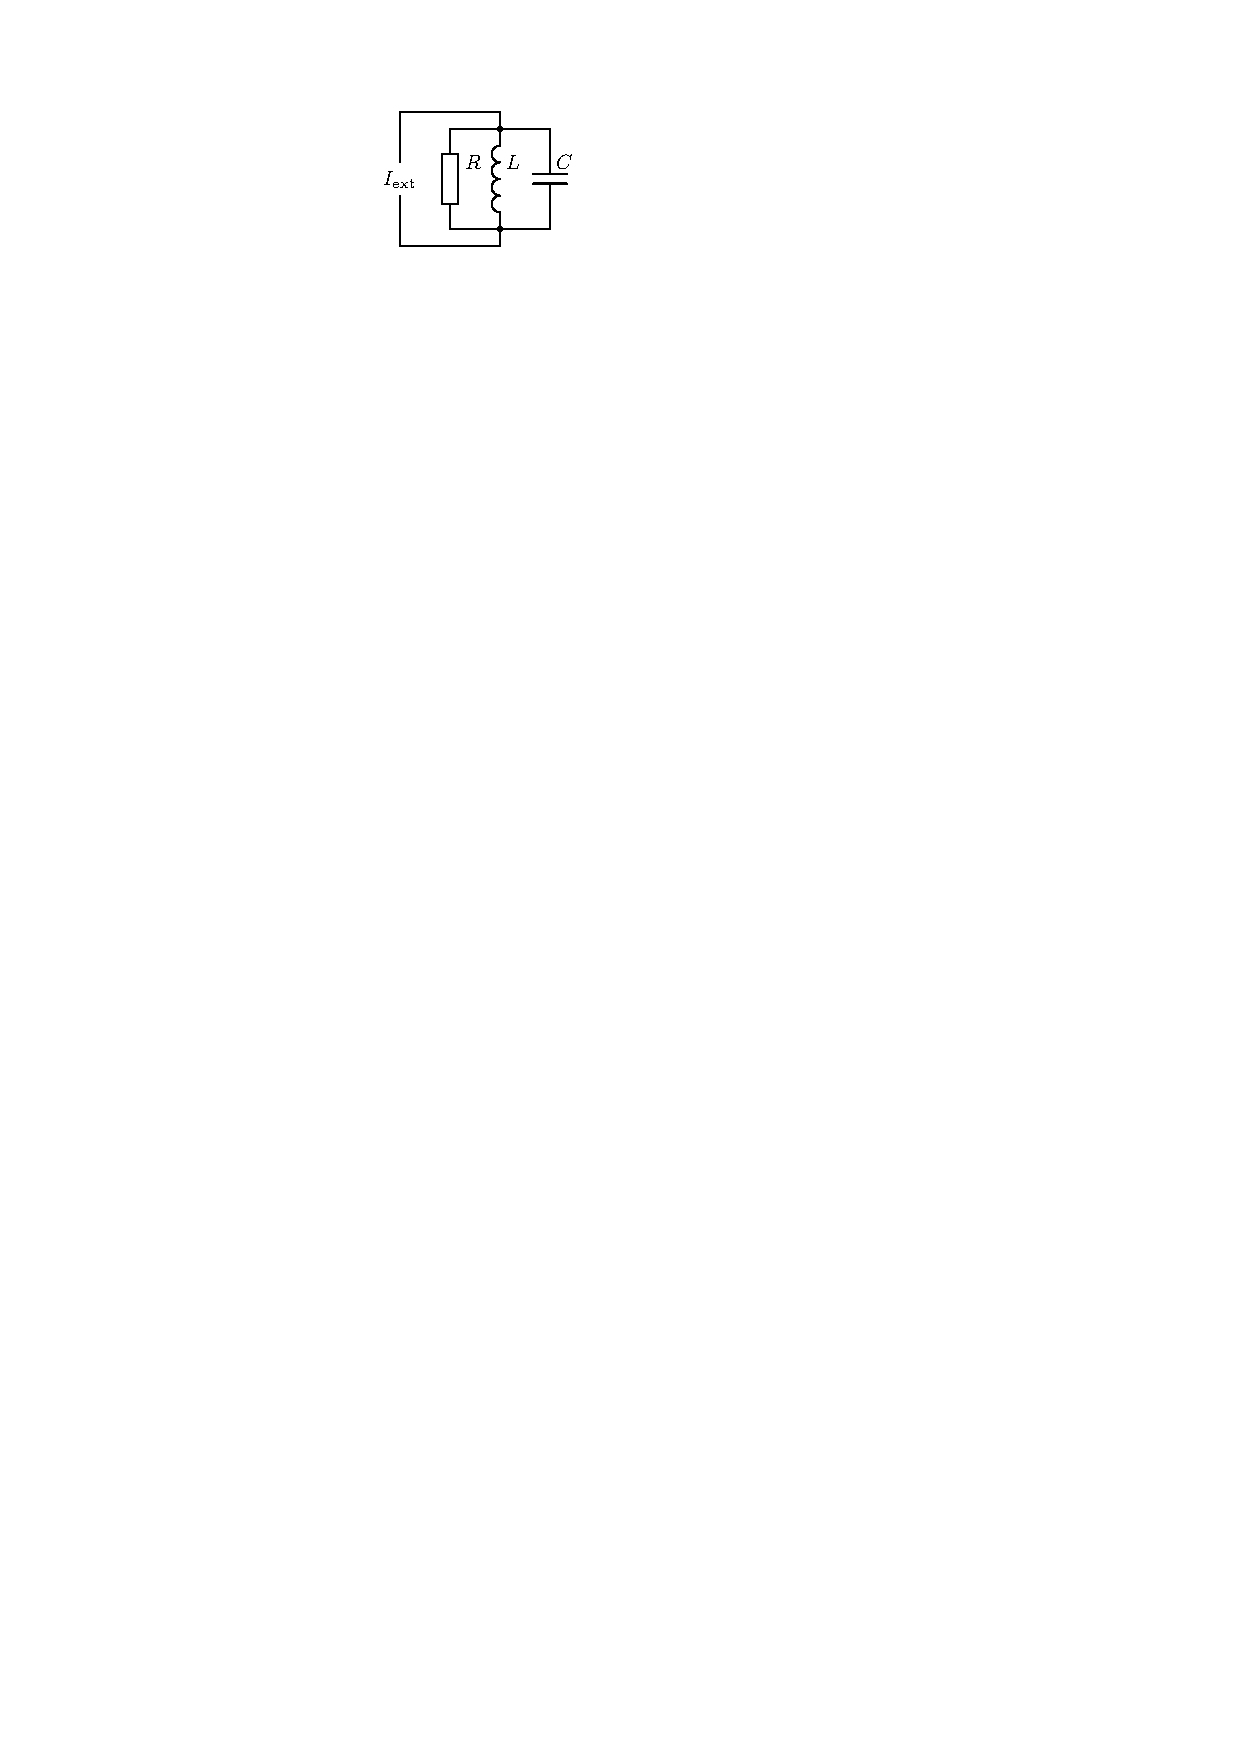
\includegraphics[width=0.35\textwidth]{./figures/RLC_circuit.pdf}
		\caption{RLC Parallelschwingkreis}
		\label{fig:rlc_circuit}
	\end{figure}
	Die elektrischen Eigenschaften von Hohlraumresonatoren in der Nähe einer Resonanz können durch das Modell des Parallelschwingkreises erklärt werden.
	Zur vollständigen Beschreibung ist die Angabe der drei Kenngrößen: Widerstand~$R$, Induktivität~$L$ und Kapazität~$C$ ausreichend.
	Für die Behandlung von Kavitäten ist es zweckmäßig andere Parameter zur Beschreibung zu verwenden.
	Dazu verwendet man die Eigenfrequenz~$\omega_0$, Kreisgüte~$Q_0$ und Widerstand~$R$ des Schwingkreises.
	Die Eigenfrequenz des Kreises folgt aus der \textsc{Thomson}schen Schwingungsgleichung \todo{Unterschied Resonanzfrequenz und Eigenfrequenz unklar}:
	\begin{align}
		\omega_0 = \frac{1}{\sqrt{L C}}
	\end{align}
	und die Kreisgüte aus ihrer Definition \todo{Definition mit Verlustleistung}:
	\begin{align}
		Q_0 &\coloneqq 2\pi \cdot \frac{\text{gespeicherte Energie}}{\text{Energieverlust pro Periode}} = \frac{\omega_0 W_0}{P_\mathrm{V}} = \omega_0 R C
		\label{eq:def_guete}
	\end{align}
	Nach der Einführung dieser Kenngrößen kann die Impedanz des Kreises beziehungsweise des Hohlraumresonators ausgedrückt werden als:
	\begin{align}
		Z(\omega) = \frac{R}{1 + i Q_0 \left( \frac{\omega}{\omega_0}  - \frac{\omega_0}{\omega}\right)}
	\end{align}
	
	Bisher war die Betrachtung auf ungetriebene Resonatoren beschränkt und soll nun auf die Anregung durch ein externes Hochfrequenzsignal erweitert werden.
	Zur Übertragung der Leistung aus einem Wellenleiter mit charakteristischer Impedanz $Z_0$ in eine Schwingungsmode der Kavität können verschiedene Methoden verwendet werden.
	Eine ist die induktive Kopplung an das Magnetfeld der Mode, bei der der Wellenleiter mit einer Leiterschleife (die sog.\ Koppelschleife) im Resonator verbunden ist.
	Dadurch wird in der Leiterschleife ein hochfrequenter Wechselstrom angeregt, welcher wiederum ein Magnetfeld erzeugt, dass Moden in der Kavität resonant anregen kann\footnote{Dies ist nur möglich wenn die jeweilige Mode am Ort der Koppelschleife ein nicht verschwindendes Magnetfeld besitzt.}.
	
	Im Modell des Parallelschwingkreises bedeutet dies, dass die Impedanz~$Z(\omega)$ der Kavität durch die induktive Kopplung transformiert wird.
	Direkt hinter der Koppelschleife habe der Resonator die transformierte\footnote{insbesondere gilt: $Z^\prime(\omega) \propto Z(\omega) \longrightarrow \frac{Z^\prime(\omega)}{Z_0} = \frac{\kappa}{R} \cdot Z(\omega)$ \todo{Hier}} Impedanz $Z^\prime(\omega)$.
	Man definiert als Maß für die Kopplung den sog.\ Koppelfaktor:
	\begin{align}
		\kappa = \frac{Z^\prime(\omega_0)}{Z_0}
		\label{eq:koppelfaktor}
	\end{align}
	mit dem Wellenwiderstand~$Z_0$ des Wellenleiters.
	Man unterscheidet zwischen unterkritischer $(\kappa < 1)$, kritischer $(\kappa = 1)$ und überkritischer Kopplung $(\kappa > 1)$.
	Im Falle von resonanter Anregung bei kritischer Kopplung folgert man aus Gleichung \eqref{eq:koppelfaktor}, dass der Wellenleiter mit seiner charakteristischen Impedanz abgeschlossen ist und somit keine Reflexionen an der Koppelschleife entstehen.
	Dies ist für den Betrieb von Beschleunigungsresonatoren wünschenswert, da dadurch die gesamte Leistung in den Resonators transmittiert wird\todo{weg?}.
	
	Von besonderem Interesse ist der komplexe Reflexionskoeffizient $\rho$, da dieser direkt mit einem vektoriellen Netzwerkanalysator messbar ist.
	Er beschreibt das Verhältnis der komplexen Spannungsamplituden von hin- und rücklaufender Welle in einem Wellenleiter.
	Aus der Leitungstheorie \cite{pozar} folgt für den Reflexionskoeffizienten am Übergang von einem Wellenleiter mit Wellenwiderstand $Z_0$ auf eine Abschlussimpedanz $Z^\prime$:
	\begin{align}
		\rho = \frac{Z^\prime - Z_0}{Z^\prime + Z_0}
		\label{eq:reflexionskoeff_trans_line}
	\end{align}
	Es folgt nach Einsetzen von () in \eqref{eq:reflexionskoeff_trans_line} der Ausdruck für den Reflexionskoeffizienten 
	\begin{align}
		\rho(\omega) = \frac{\frac{\kappa}{R} \cdot Z(\omega) - 1}{\frac{\kappa}{R} \cdot Z(\omega) + 1} = \frac{(\kappa - 1) + i  Q_0 \left( \frac{\omega}{\omega_0}  - \frac{\omega_0}{\omega}\right)}{\left( \kappa + 1 \right) + i  Q_0 \left( \frac{\omega}{\omega_0}  - \frac{\omega_0}{\omega}\right)}
	\end{align}
	\todo{Abschlusssatz}

	\section{Resonante Störkörpermessung}
	\todo{Vernachlässigung von Luft $\mu$, $\epsilon$}
	Die resonante\footnote{\todo{Was ist nicht resonante SKM?}} Störkörpermessung basiert auf der Störung eines Hohlraumresonators durch einen dielektrischen oder magnetischen Körper (dem sog.\ Störkörper), welcher durch das Feld im Resonator polarisiert beziehungsweise magnetisiert wird.
	Eine solche lokalisierte Störung verursacht eine Verschiebung der Resonanzfrequenz~$\Delta \omega$ in Abhängigkeit des elektrischen und magnetischen Feldes am Ort des Störkörpers.
	Quantitativ kann die Verschiebung beschrieben werden durch (für eine Herleitung siehe Anhang \ref{app:herleitung_frequenzverschiebung}):
	\begin{align}
		\frac{\Delta \omega}{\omega_0} = - \frac{\int_V \mathrm{d}V \left[ \ve_0^* \cdot \vec{P} + \vb_0^* \cdot \vec{M} \right]}{4 W_0}
		\label{eq:frequenzverschiebung}
	\end{align}
	mit dem Resonatorvolumen~$V$, der Polarisation~$\vec{P}$, der Magnetisierung~$\vec{M}$, der im elektromagnetischen Feld gespeicherten Energie~$W_0$ und den komplex konjugierten Feldern $\ve_0^*, \vb_0^*$ des ungestörten Resonators.
	
	Im Rahmen dieser Arbeit wird eine dielektrische Kugel mit relativer elektrischer Permittivität~$\epsilon_\mathrm{r}$ verwendet.
	Darüber hinaus sei die magnetische Permeablität~$\mu$ vernachlässigbar, sodass es zu keiner Magnetisierung ($\vec{M} = 0$) des Störkörpers kommt.
	Weiterhin wird angenommen, dass das Volumen des kugelförmigen Störkörpers wesentlich kleiner ist als das Resonatorvolumen, sodass am Ort des Störkörpers das elektrische Feld als homogen angesehen werden kann.
	Dadurch kann die Polarisation $\vec{P}$ der dielektrischen Kugel im homogenen elektrischen Feld $\ve_0$ ausgedrückt werden als \cite{jackson}:
	\begin{align}
		\vec{P} = 3 \, \frac{\epsilon_\mathrm{r} - 1}{\epsilon_\mathrm{r} + 2} \, \epsilon_0 \ve_0
		\label{eq:polarisation_kugel}
	\end{align}
	mit der elektrischen Feldkonstante~$\epsilon_0$.
	Durch die Annahme der Homogenität der Felder und verschwindender Polarisation und Magnetisierung außerhalb des Störkörpervolumens~$V_\mathrm{s}$ kann direkt crcdie Amplitude $|\ve_0|$ des elektrischen Feldes am Ort des Störkörpers berechnet werden:\todo{Übergang unklar, vorallem was Positionsabhängigkeit der Felder angeht und Verschwindender Polarisation/Magnetisierung im Resonatorvolumen, negatives Vorzeichen in der Wurzel}
	\begin{align}
		|\ve_0| = \sqrt{-4 \cdot \frac{W_0}{\alpha_\mathrm{s}} \cdot \frac{\Delta \omega}{\omega_0}} \label{eq:skm_e_feld}
	\end{align}
	wobei man die sogenannte Störkörperkonstante $\alpha_\mathrm{s}$ definiert:
	\begin{align}
		\alpha_\mathrm{s} \coloneqq 3 \, \frac{\epsilon_\mathrm{r} - 1}{\epsilon_\mathrm{r} + 2} \, \epsilon_0 V_\mathrm{s}
	\end{align}
	Die Amplitude des elektrischen Feldes in Gleichung \eqref{eq:skm_e_feld} ist von der im Resonator gespeicherten Energie $W_0$ abhängig, welche wiederum von der in den Resonator eingekoppelten Leistung abhängt.
	Daher ist es zweckmäßig die gespeicherte Energie $W_0$ über Gleichung \eqref{eq:def_guete} in abhängigkeit der Güte $Q_0$ und Verlustleistung $P_\mathrm{V}$ auszudrücken.
	Die Amplitude des elektrischen Feldes kann dann auf die Wurzel der Verlustleistung normiert werden und man erhält:
	\begin{align}
		\frac{|\ve_0|}{\sqrt{P_\mathrm{V}}} = \sqrt{-4 \cdot \frac{Q_0}{\alpha_s} \cdot \frac{\Delta \omega}{\omega_0^2}}
	\end{align}	
	
	\chapter{Störkörpermessung}
	Permittivität Teflon \cite{CRC} $\epsilon_\mathrm{r} = \num{2.1}$.
	Berechnen der Störkörperkonstante \todo{Fehler ist noch nicht richtig!}:
	\begin{align}
		\alpha_\mathrm{s} = \SI{2.985 +- 0.1e-17}{\ampere\second\metre\squared\per\volt}
	\end{align}


	
	Mit dem Betrag:
	\begin{align}
		| \rho(\omega) | = \sqrt{\frac{(\kappa - 1)^2 + Q_0^2 \left( \frac{\omega}{\omega_0}  - \frac{\omega_0}{\omega}\right)^2}{(\kappa + 1)^2 + Q_0^2 \left( \frac{\omega}{\omega_0}  - \frac{\omega_0}{\omega}\right)^2}}
	\end{align}
	\begin{figure}[ht]
		\centering
		\input{./plots/outfile.tex}
		\caption{Gütefit}
		\label{fig:gütefit}
	\end{figure}
	
	
	
	
	\chapter{Fazit}
	     
	\appendix
	\chapter{Herleitung der Frequenzverschiebung bei Störkörpermessung}
	\label{app:herleitung_frequenzverschiebung}
	Man betrachte das zeit- und ortsabhängige elektromagnetische Feld in einem Hohlraumresonators, charakterisiert durch elektrische Feldstärke~$\ve$ und magnetische Feldstärke~$\vh$.
	Die Felder des ungestörten Resonators seien gegeben durch $(\ve_0, \vh_0)$ und die des gestörten Resonators durch $(\ve_1, \vh_1)$.
	Bei Verwendung der komplexen Darstellung der stehenden Welle im Resonator, kann das elektromagnetische Feld angegeben werden als:
	\begin{subequations}
		\label{eq:skm_felder}
		\begin{align}
		&\ve_{0,1}(x,y,z,t) = \ve_{0,1}(x,y,z) \, e^{i \omega_{0,1} t}\\
		&\vh_{0,1}(x,y,z,t) = \vh_{0,1}(x,y,z) \, e^{i \omega_{0,1} t}
		\end{align}
	\end{subequations}
	wobei die Phasenbeziehung von elektrischem und magnetischem Feld in den komplexen Amplituden $\ve_{0,1}(x,y,z)$ und $\vh_{0,1}(x,y,z)$. enthalten ist.
	Unabhängig von der Störung des Feldes gelten die \textsc{Maxwell}-Gleichungen \cite{jackson}:
	\begin{subequations}
		\label{eq:skm_maxwell}
		\begin{align}
			\vnabla \times \ve &= - \frac{\partial \vb}{\partial t}\\
			\vnabla \times \vh &= \vec{j}_\mathrm{frei} + \frac{\partial \vd}{\partial t}
		\end{align}
	\end{subequations}
	Setzt man die gestörten und ungestörten Felder \eqref{eq:skm_felder} in die \textsc{Maxwell}-Gleichung \eqref{eq:skm_maxwell} ein, so erhält man unter der Annahme einer verschwindenden freien Stromdichte $\vec{j}_\mathrm{frei}$ im Hohlraum und nach Elimination der Zeitabhängigkeit:
	\begin{subequations}
		\label{eq:skm_zeitunabhaengig}
		\begin{align}
			&\vnabla \times \ve_{0,1} = - i \omega_{0,1} \vb_{0,1} \\
			&\vnabla \times \vh_{0,1} = i \omega_{0,1} \vd_{0,1}
		\end{align}
	\end{subequations}
	Man verwendet diese zeitunabhängigen Gleichungen und die Produktregel der Divergenz für das Kreuzprodukt um die folgenden Identitäten zu finden:
	\begin{subequations}
		\label{eq:skm_vektoridentitaeten}
		\begin{align}
		\vnabla \cdot \left( \ve_0^* \times \vh_1\right) &= \vh_1 \cdot \left( \vnabla \times \ve_0^* \right) - \ve_0^* \cdot \left( \vnabla \times \vh_1 \right) \nonumber \\
		&= i \omega_0 \vb_0^* \vh_1 - i \omega_1 \ve_0^* \vd_1 \label{eq:e0h1} \\[0.5em]
		%
		\vnabla \cdot \left( \ve_1 \times \vh_0^* \right) &= \vh_0^* \cdot \left( \vnabla \times \ve_1 \right) - \ve_1 \cdot \left( \vnabla \times \vh_0^* \right) \nonumber \\
		&= i \omega_0 \ve_1 \vd_0^* - i \omega_1 \vb_1 \vh_0^* \label{eq:e1h0}
		\end{align}
	\end{subequations}
	Anschließend bildet man die Summe der Gleichungen \eqref{eq:skm_vektoridentitaeten} und führt eine Integration über das Resonatorvolumen $V$ durch.
	Unter Verwendung des \textsc{Gauß}schen Integralsatzes erhält man:
	\begin{align}
		\int_{V} \mathrm{d}V \left[ \vnabla \cdot \left( \ve_0^* \times \vh_1 + \ve_1 \times \vh_0^* \right) \right] = \oint_{\partial V} \mathrm{d}S \left[ \vec{n} \cdot \left( \ve_0^* \times \vh_1 + \ve_1 \times \vh_0^* \right)\right] \label{eq:volint}
	\end{align}
	wobei $\vec{n}$ den Normaleneinheitsvektor auf dem Rand $\partial V$ des Resonatorhohlraums darstellt.
	Die Randbedingungen für das elektrische und magnetische Feld am idealen Leiter \eqref{eq:randbedingung_leiter} sorgen dafür, dass das Skalarprodukt im Integranden der rechten Seite auf dem Rand des Volumens $\partial V$ identisch verschwindet\footnote{Das Kreuzprodukt von elektrischer und magnetischer Feldstärke steht stehts senkrecht zum Normalenvektor der ideal leitenden Grenzfläche: $\ve \times \vh \perp \vec{n}$}.
	Setzt man die gefundenen Identitäten \eqref{eq:skm_vektoridentitaeten} in das Integral über das Resonatorvolumen ein, so erhält den Zusammenhang zwischen ungestörter~$\omega_0$ und gestörter Resonanzfrequenz~$\omega_1$:
	\begin{align}
		\omega_0 \int_{V} \mathrm{d}V \left( \vb_0^* \cdot \vh_1 + \ve_1 \cdot \vd_0^* \right) = \omega_1 \int_{V} \mathrm{d}V \left( \vb_1 \cdot \vh_0^* + \ve_0^* \cdot \vd_1 \right)
	\end{align}
	Dieser Zusammenhang ermöglicht es einen Ausdruck ermöglicht die Angabe der relativen Frequenzverschiebung:
	\begin{align}
		\frac{\Delta \omega}{\omega_0}= \frac{\omega_1 - \omega_0}{\omega_0} = \frac{\int_{V} \mathrm{d}V \left[ \left( \ve_1 \cdot \vd_0^* - \ve_0^* \cdot \vd_1 \right) + \left( \vb_0^* \cdot \vh_1 - \vb_1 \cdot \vh_0^* \right)\right]}{\int_V \mathrm{d}V \left[\ve_0^* \cdot \vd_1 + \vb_1 \cdot \vh_0^* \right] }
		\label{eq:skm_rel_freqabweichung_schritt}
	\end{align}
	Unter Verwendung der Definitionen für die magnetische Feldstärke $\vh$ und der elektrischen Flussdichte $\vd$:
	\begin{subequations}
		\begin{align}
			&\vd \coloneqq \epsilon_0 \ve + \vec{P}\\
			&\vh \coloneqq \frac{1}{\mu_0} \vb - \vec{M}
		\end{align}
	\end{subequations}
	mit den Vektorfeldern der Polarisation $\vec{P}$ und Magnetisierung $\vec{M}$ folgt aus \eqref{eq:skm_rel_freqabweichung_schritt}:
	\begin{align}
		\frac{\Delta \omega}{\omega_0} = - \frac{\int_V \mathrm{d}V \left[ \ve_0^* \cdot \vec{P} + \vb_0^* \cdot \vec{M} \right]}{\int_V \mathrm{d}V \left[ \ve_0^* \cdot \vd_1 + \vb_1 \cdot \vh_0^* \right]} \label{eq:skm_rel_freqabweichung_schritt2}
	\end{align}
	Schließlich wird angenommen, dass das Volumen des Störkörpers klein ist gegen das gesamte Resonatorvolumen.
	Dadurch können bei Integration über das Resonatorvolumen im Nenner von \eqref{eq:skm_rel_freqabweichung_schritt2}, die gestörten Felder im Integranden durch die Ungestörten genähert werden.
	Beachtet man weiterhin, dass die Phasendifferenz von elektrischem und magnetischem Feld bei stehenden elektromagnetischen Wellen $\pi / 2$ beträgt, so erhält man nach Ausführen der Integration im Nenner die vierfache im Feld des Resonators gespeicherte Energie~$W_0$:
	\begin{align}
		\frac{\Delta \omega}{\omega_0} = - \frac{\int_V \mathrm{d}V \left[ \ve_0^* \cdot \vec{P} + \vb_0^* \cdot \vec{M} \right]}{4 W_0}
	\end{align}
	Diese Gleichung verknüpft die Verschiebung der Resonanzfrequenz durch einen Störkörper mit den ungestörten elektrischen und magnetischen Feldern und ermöglicht die Messung der Felder bei geeigneter Wahl des Störkörpers.
	\todo{Frequenzverschiebung ist negativ}
		
	\backmatter
		
	\begin{thebibliography}{19}
	\bibitem{hillert}
		\textsc{W.\ Hillert},
		\emph{E 106: Cavities, Details on the experimental method}, Bonn, 2008.

	\bibitem{wangler}
		\textsc{T.\ P.\ Wangler},
		\emph{Principles of RF Linear Accelerators},
		Wiley, New York, 1998.
	
	\bibitem{pozar}
		\textsc{D.\ M.\ Pozar},
		\emph{Microwave Engineering}, 4.\ Auflage,
		Wiley, New York, 2011.
	
	\bibitem{jackson}
		\textsc{J.\ D.\ Jackson},
		\emph{Classical Electrodynamics}, 1.\ Auflage,
		Wiley, New York, 1962.
	
	\bibitem{CRC}
		\textsc{D.\ R.\ Lide} (Hrsg.),
		\emph{CRC Handbook of Chemistry and Physics}, 90. Auflage,
		CRC Press, Florida, 2010.
		
	
	\end{thebibliography}
	
	\chapter{Danksagung}
	
	\listoffigures
	\listoftables
	
\end{document}
